\section{Methodology and Design}

\subsection{Design Process}

The Search \& Support Fleet Robotics team is implementing a rigorous design process for all aspects of this project's design. The team aims to deliver the best possible product within the given time and budget constraints. Due to these constraints, the team will rely heavily on inexpensive, quickly created design prototypes. The team’s design process is as follows:

\begin{enumerate}
    \item As a group, brainstorm the \nameref{sec:mvp} and \nameref{sec:sg} for the design at hand.  
    Example: The MVP's \gls{gui} is simple and functional, with the stretch goal of makings it look nice.  

    \item Complete research to determine the best fit for the team’s needs. The department lead will complete the majority of the research, but all team members will assist/challenge their findings.  
    Example: Creating a decision matrix, as seen in Table~\ref{tab:decision_matrix}.  

    \item The mechanical-focused team member will create a rough sketch/design, and the rest of the team will constructively criticize it, whilst brainstorming if anything is missing.  
    Example: \gls{gui} design drawn on paper, showing the placement of buttons and other controls.  

    \item Once all members have agreed on a rough sketch/design, the department lead has the green light to start on the prototype.  
    This will be a cheap prototype, such as using cardboard for mechanical design or PowerPoint for the \gls{gui} design.  

    \item The first iteration of the prototype will be tested by team members as well as external volunteer testers, if applicable.  

    \item The feedback gathered from the testing will be used in creating the next iteration.  

    \item Steps 5 and 6 will repeat until the team is confident in the current prototype iteration.  

    \item When the iteration has been approved, the prototype will be built more thoroughly.  
    This means a more solid prototype, such as using wood/plastic for a mechanical design and coding out a rough \gls{gui}.  

    \item This stage, if all team members approve of the prototype, one member will complete a test matrix, created by the department lead, ensuring all functionality and proper design fit. If applicable, the test matrix will also be completed by external volunteer testers.  

    \item The final product will be built from the successful prototype and then will go through another test matrix to iron out any last issues.
\end{enumerate}
\begin{table}[H]
    \centering
    \caption{Weighted decision matrix comparing potential drivetrain and chassis configurations \cite{wong2006wheels}}
    \begin{tabular}{|p{3cm}|c|c|c|c|c|c|c|}
        \hline
        \textbf{Criteria} & \textbf{Weight} & \textbf{\shortstack{Skid\\Steering}} & \textbf{\shortstack{Diff.\\Drive}} & \textbf{\shortstack{4x4\\Wheeled\\Ackermann}} & \textbf{Tracked} & \textbf{\shortstack{Cntr.\\Art.\\Wheeled}} & \textbf{\shortstack{Cntr\\Art.\\Tracked}} \\

        \hline
        Maneuverability & 0.20 & 4 & 3 & 2 & 4 & 5 & 4 \\
        \hline
        Stability on uneven terrain & 0.20 & 3 & 2 & 3 & 5 & 4 & 4 \\
        \hline
        Traction & 0.20 & 4 & 2 & 3 & 5 & 4 & 5 \\
        \hline
        Payload capacity & 0.20 & 3 & 2 & 4 & 4 & 5 & 5 \\
        \hline
        Robustness & 0.10 & 4 & 3 & 3 & 4 & 3 & 4 \\
        \hline
        Speed / Efficiency & 0.10 & 3 & 4 & 5 & 2 & 3 & 2 \\
        \hline
        \textbf{Score} & \textbf{1} & \textbf{3.50} & \textbf{2.50} & \textbf{3.20} & \textbf{4.20} & \textbf{4.20} & \textbf{4.20} \\
        \hline
    \end{tabular}

    \label{tab:decision_matrix}
\end{table}

\subsection{System Architecture}

The system architecture of the Search \& Support Fleet Robotics project is split into two main components: the development environment and the autonomous robot platform, as shown in Figure~\ref{fig:system_architecture}.

\textbf{The development environment} consists of a laptop running Ubuntu 24.04. ROS2 Jazzy Jalisco and Gazebo Harmonic simulate the robot in mining settings. During the design process, ROS2 will also assist with processing data from the robot. The Arduino IDE is used for calibrating and validating sensors and actuators before integrating them into the robot. VS Code and Remmina provide tools for remote access and development. This environment enables the team to design, simulate, and validate system functionality before deployment to the physical robot.

\textbf{The autonomous robot platform} comprises onboard computing, sensing, and actuation subsystems. A Raspberry Pi 5 running Ubuntu 24.04 is the primary compute of the platform. ROS2 Jazzy Jalisco manages localization, navigation, and sensor integration for the robot. Complementing this, an Arduino UNO R4 Wi-Fi connected via Micro ROS provides motor control and sensor interfacing. The Arduino’s serial monitor can be accessed directly through the Arduino CLI. A \gls{lidar} sensor provides mapping and anomaly detection, while ultrasonic sensors handle short-range obstacle avoidance. Localization functionality is based on the encoder and \gls{imu} data. Human detection is accomplished by an \gls{ir} temperature sensor, with a camera and microphone reserved for future implementation as part of the \nameref{sec:sg}. Environmental conditions are monitored using multi-gas sensors, as well as temperature and humidity sensors.

\begin{figure}[H]
    \centering
    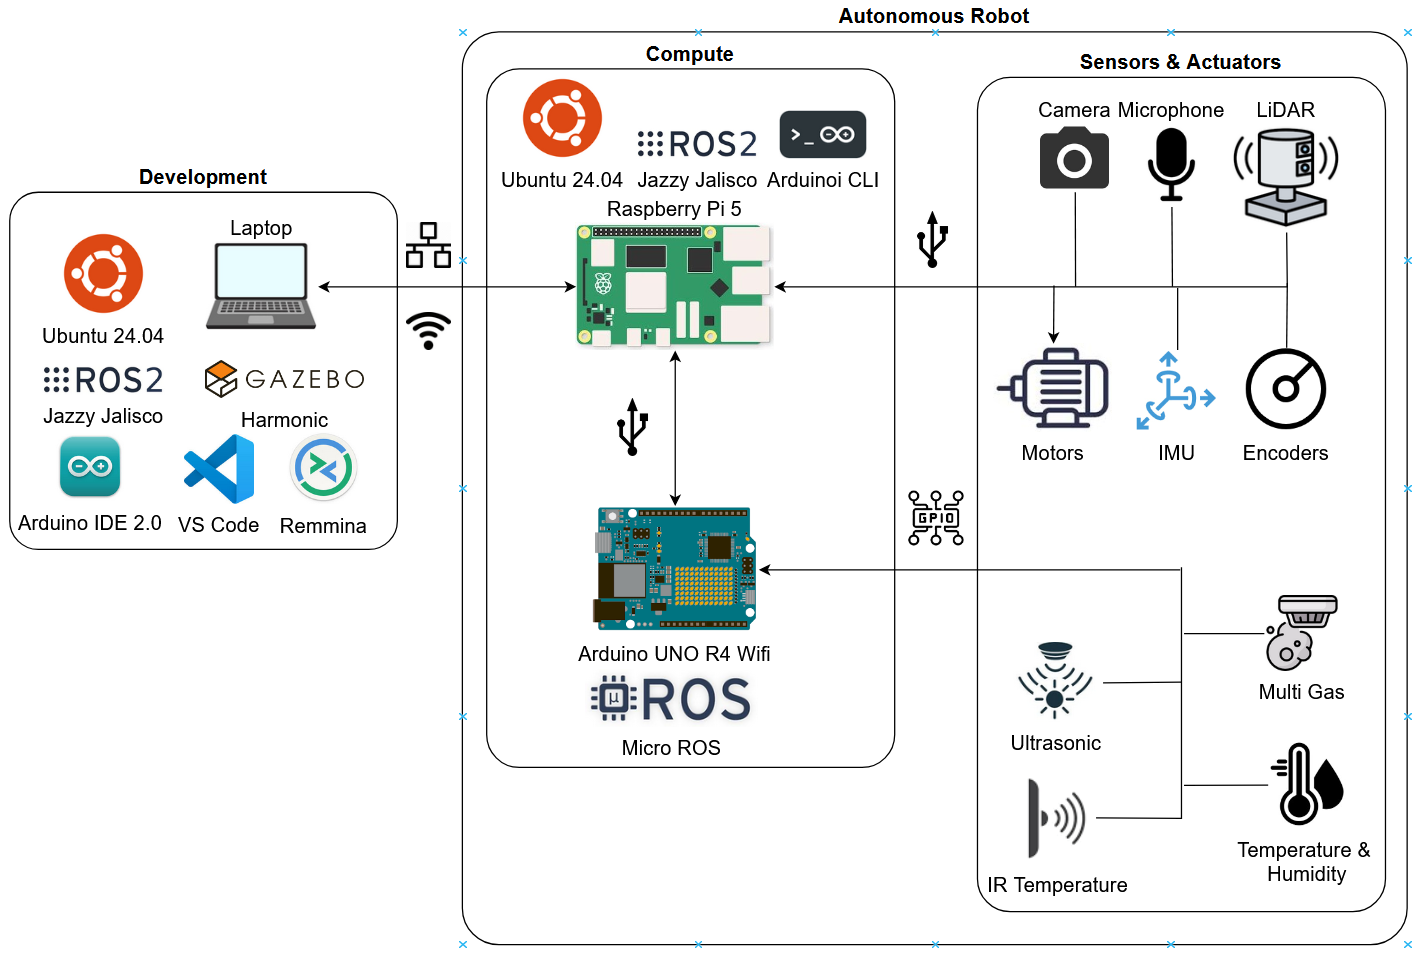
\includegraphics[width=0.9\textwidth]{images/system_archietecture.png}
    \caption{System diagram including the autonomous robot and development laptop.}
    \label{fig:system_architecture}
\end{figure}

\subsection{Validation Tools and Resources}

To validate the proposed system, the team has defined the following test plans.

\textbf{The navigation system} will be validated utilizing a simulated environment in Gazebo, in addition to a physical test using the prototype chassis. In these tests, the team will measure the success rate of obstacle avoidance, speed, and localization drift using ROS2 logs (see the \nameref{sec:requirements} section).

\textbf{The human detection system} will be validated by integrating the \gls{ir} sensor in a controlled environment, with team members at varying distances and levels of occlusion. The robot will attempt to detect any human presence, and its performance will be evaluated based on detection accuracy, false positive/negative rates, and detection time. ROS2 logs, alongside video recording, will be used to analyze the results.

\textbf{The environmental sensing system} will be evaluated utilizing accessible baseline tests. Temperature and humidity sensors will be exposed to various real-world conditions, and the team will confirm that the readings change as expected. The performance of gas sensors will be evaluated by monitoring the output when exposed to breath (CO2 detection). Data will be captured and analyzed using ROS2 logs and the Arduino serial monitor. Although precise calibration cannot be performed, these tests will provide a baseline functionality to enable integration into the robotic platform. 

\textbf{The autonomous drivetrain performance} will be tested with and without the desired payload to understand the effect of the added weight. The test manoeuvres include:
\begin{itemize}
    \item Straight line speed runs
    \item Tight turning test
    \item Braking distance trials
    \item Ramp ascents and descents (varying slopes)
    \item Climb test
\end{itemize}

ROS2 logs will be used to capture key metrics, including maximum speed, stopping distance, turning radius, maximum slope angle, maximum obstacle height cleared, and motor temperature.

\textbf{The reliability of communication} will be tested by connecting a Raspberry Pi 5 and ESP modules in a controlled environment. Wireshark will be used to compare the signal strength, latency, bandwidth, and packet loss at increasing distances and with obstacles between each unit.